\documentclass[]{vgtuef}
\usepackage[utf8x]{inputenc}
\usepackage[L7x]{fontenc}
\usepackage[lithuanian]{babel}

\author{Tomas Fedosejev, Marius Buinevičius\\Vilniaus Gedimino technikos
  universitetas\\Elektronikos fakultetas\\Elektroninių sistemų
  katedra\\\texttt{tomas@fedosejev.lt}}
\title{Bakalauro baigiamasis darbas\\Virtualios garso realybės sistema}


\begin{document}

\setcounter{page}{7}

\onehalfspacing

\tableofcontents


\section*{Žymenys ir santrumpos}
\addcontentsline{toc}{section}{Žymenys ir santrumpos}

\begin{itemize}
\item HRTF - su galva susijusios perdavimo funkcijos (angl. \textit{Head Related Transfer Function}).
\item ATF - anatominė perdavimo funkcija (angl. \textit{Anatomical Transfer Function}).
\item FFTF - (angl. \textit{Field-Free Transfer Function}).
\item RIR - kambario impulsinis atsakas (angl. \textit{Room Impulse Response}).
\item HRIR - (angl. \textit{Head Related Impulse Response}).
\item ITD - tarpausinis laiko skirtumas (angl. \textit{Interaural Time Difference}).
\item ILD - tarpausinis garso lygių skirtumas (angl. \textit{Initial Level Difference}).
\item USB - universalioji nuoseklioji jungtis (angl. \textit{Universal Serial Bus}).
\item COM - RS232 nuoseklusis prievadas.

\end{itemize}


\section{Įvadas. Užduoties analizė}

Baigiamasis bakalaurinio baigiamojo darbo tema: „Virtuali garso realybės sistema“. Šiuo darbu siekiama ištirti galimybes bei sukurti realiuoju laiku veikiančia sistemą gebančią generuoti binauralinį garsą priklausomai nuo vartotojo galvos orientacijos ir virtualios aplinkos parametrų.
Baigiamojo bakalaurinio darbo sistemos vartotojo sąsajos programinei įrangai reikalingi mažiausiai 20MB diskinio kaupiklio dalies talpos. Toks atminties kiekis reikalingas norint vartotojo sąsają padaryti patrauklesnę vartotojui, t.y. grafinės iliustracijos, garsai ir kt.
Vartotojo sąsajos programinė įranga dirba Windows 7 operacinėje sistemoje, nes senesnės versijos \textit{(XP, Vista)} jau yra nebepalaikomos Microsoft korporacijos.
\textit{USB} lizdo versija negali būti mažesnė nei 1.1, nes sistema suprojektuota darbui su šia ar aukštesnėmis versijomis. Duomenų perdavimą taipogi būtų galima realizuoti ir kitomis sąsajomis, tokiomis kaip \textit{COM}, bet tokiu atveju greitis būtų nepakankamas ir sistema įgautų netoleruotiną vėlinimą. Be to, binauralinio garso generavimo sistema yra šiuolaikinė ir labiau taikintina nešiojamiems kompiuteriams, kuriuose nebediegiami \textit{RS232} prievadai. Išlieka galimybė naudoti \textit{RS232} prievadą, bet tokiu atveju tektų papildomai turėti iš \textit{USB} į \textit{COM} keitiklio kabelį, kuris taip pat naudoja \textit{USB} jungtį. Todėl geriausias pasirinkimas spartos atžvilgiu rinktis virtualų \textit{COM} prievadą per \textit{USB} jungtį.
Siekiant išlaikyti kuriamos sistemos kuo ilgesnį gyvavimo laiką be įkrovimo sistema toleruoja maksimalų 0,5 A srovės suvartojimą (tiek galvos orientacijos nustatymo įrenginys tiek garso apdorojimo įrenginys), be to 0,5 A tai didžiausia srovė kurią pagal specifikaciją gali atiduoti\textit{USB} 1.1 ir \textit{USB} 2.0 prievadai.
Norint išlaikyti sistemos mobilumą, kurio didžioji dalis priklauso nuo galvos sekimo įrenginio dydžio, buvo pasirinkti pakankamai nedideli pastarojo įrenginio matmenys: 50 × 100 × 100 mm.  

\section{Analogiškų sistemų apžvalga}

Šiame skyriuje bus apžvelgtos analogiškos sistemos: buvę prototipai ir šiuo metu esami rinkoje produktai. Apibendrintai bus aptarti nagrinėjamų sistemų teigiamos ir neigiamos savybės. 


Galvos sekimo įrenginio kūrimas nėra naujiena. Tokie įrenginiai naudojami norint nusakyti lėktuvų  trimatę poziciją. Pati \textit{sensor fusion} technologija taip pat jau gana ilgai naudojama aviacijos srityje, norint kur kas tiksliau nusakyti poziciją.
Kalbant apie binauralinio garso generavimą realiu laiku, paieškos rezultatai stipriai sumažėja. Tokio tipo projektų pasaulyje yra tik du. Projekto tikslai – binauralinio garso generavimas realiu laiku. Vienas iš projektų naudojo \textit{„Texas instruments“} pagamintą plokštę - C6713 DSK kuri pavaizduota \ref{fig:C6713_dsk_board} pav.

\begin{figure}[!h]
  \centering
  \includegraphics[width=400px]{img/c6713.jpg}
  \caption{C6713 DSK spausdintinė plokštė.}
  \label{fig:C6713_dsk_board}
\end{figure}

Šios plokštės mikrovaldiklis dirba 225 MHz dažniu ir pasiekiantis 1800 milijonų instrukcijų per sekundę spartą. Taip pat ši plokštė gali apdoroti aukštos kokybės 24 bitų skaitmeminį stereo garsą, turi 512 kB \textit{Flash} bei 16 MB \textit{SDRAM} atmintis. \textit{JTAG}\footnote{JTAG - Programavimo ir testavimo jungtis.} prieinamas per \textit{USB} jungtį.

Kaip teigia gaminio kūrėjai, jie generuoja binauralinį garsą naudojant specialų stereo filtrą suprogramuotą minėtoje plokštėje. Programinė įranga naudoja nuo galvos priklausančias impulso atsako funkcijas sugeneruotas \textit{„Floridos tarptautinio universiteto“} asmenų (nepaminėta kieno). Dviejų kanalų išėjimui panaudotos 12 \textit{HRTF} funkcijų, kurios taip pat nebuvo sugeneruotos projekto autorių. 

Kūrėjų teigimu, rezultatai jų stipriai nestebina – geriausias efektas jaučiamas tik garsui esant už galvos, nes panaudotos \textit{HRTF} funkcijos nėra pritaikytos jų ausims. Šio įrenginio testavimo akimirką demonstruoja \ref{fig:C6713_dsk_board_checkout} pav.

\begin{figure}[!h]
  \centering
  \includegraphics[width=400px]{img/c6713_patikra.jpg}
  \caption{C6713 DSK plokštės patikra.}
  \label{fig:C6713_dsk_board_checkout}
\end{figure}


Kompiuterinis binauralinio garso generavimas yra įmanomas, bet reikalauja didelių kompiuterio resursų, taip atimdamas galią iš centrinio procesoriaus, todėl kuriamos išorinės garso plokštės, kurios nepriklausomai nuo kompiuterio procesoriaus gali generuoti binauralinį garsą naudojant \textit{HRTF} funkcijas.

Pirmoji garso rinkoje pasirodęs produktas galėjęs pasiūlyti trimatį pozicinį garso generavimą buvo 1998 išleista \textit{„Aureal Vortex via the A3D API“} garso plokštė. Deja nėra  galimybės jos išbandyti, bet pagal vartotojų atsiliepimus ši plokštė sugebėdavo gana gerai suformuoti trimačio garso pojūtį. Kadangi įmonė \textit{„Aureal“} pasitraukė iš rinkos, tai jos poziciją perėmė \textit{„Creative Inc.“} firma. Gerą garso kokybę bei neblogą trimačio garso efektą gali pasiūlyti tik labai brangios pastarosios įmonės garso plokštės – \textit{„X-Fi“}. 

Šiuo metu binauralinio garso generavimas realiu laiku priklausomas nuo vartotojo galvos pozicijos neturi jokių analogų. Kaip ir buvo minėta, atskirai abi dalys yra daugiau ar mažiau naudojamos pasaulinėje rinkoje, bet būtent šių dviejų sričių sujungimas yra visiškai unikalus, todėl analogiškų sistemų apžvalga čia yra neįmanoma.

Kaip buvo minėta apžvalgoje sistema pasiūlytame pavidale yra unikali ir perspektyvi. Šiuo metu rinkoje nėra įrenginių gebančių sugeneruoti bunauralinį garsą priklausomai nuo klausytojo galvos orientacijos. Rinkoje esantys analogai suteikia programuotojams galimybę įgyvendinti šį efektą naudojantis papildomais programiniais įrankiais, tačiau įrenginių gebančių tai padaryti savaime, be papildomo programuotojų įsikišimo - nėra.

\section{Naudojamų metodų apžvalga}

Šiame skyriuje bus apžvelgti metodai kuriais remiantis buvo sukurti matematiniai modeliai ir realios sistemos prototipas.

\subsection{HRTF funkcijos}

\textit{HRTF} (angl. \textit{Head Related Transfer Function}) dar vadinamos \textit{ATF} (angl. \textit{Anatomical Time Difference}) tai funkcijos nusakančios atsaką kurį kuris charakterizuoja, kaip žmogaus ausis priima garsą sklindantį iš tam tikro taško erdvėje. Panaudojus \textit{HRTF} porą, skirta kiekvienai ausiai, įmanoma sintezuoti binauralinį garsą taip sukuriant erdvės pojūtį.  
Žmogaus smegenys apskaičiuoja garso šaltinio poziciją erdvėje naudojantis: 1) garso užuominomis atkeliavusiomis į kiekvieną ausį (angl. \textit{monoaural cues}), 2) abiejų ausų garso užuominų palyginimu (angl. \textit{difference cues} arba \textit{binaural cues}). Pagrindinės garso užuominos yra:
\begin{enumerate}
\item Tarpausinis laiko skirtumas (angl. \textit{Interaural Time Difference})
\item Tarpausinis garso lygių skirtumas (angl. \textit{Interaural Level Difference})
\item Spektriniai skirtumai (angl. \textit{Spectral cues} arba \textit{Pinae effect})
\item Galvos šešėlis (angl. \textit{Head Shadow})
\item Pečių aidas (angl. \textit{Shoulder Echo})
\item Ankstyvieji atspindžiai (angl. \textit{Early Reflections})
\item Atgarsiai (angl. \textit{Reverberation})
\end{enumerate}

\textit{HRTF} aprašo tik dalį iš aukščiau pateiktų užuominų: TLS ir TGLS.


\subsection{Galvos šešėlis ir pečių aidas}

Galvos šešėlis arba dar kitaip vadinamas akustiniu šešėliu, tai sumažėjusios garso amplitudės regionas atsirandantis, nes galva sugeria arba sumažina amplitudę dalies ją pasiekusių garso bangų. Pasiekusi galvą garso banga gali keliauti aplink arba per galvą, kad pasiektų ausį esančią priešingoje pusėje. Tokiu būdu yra sukuriamas pakankamai geras pirminės lokalizacijos filtras. Ausį esančią šešėlyje garsas pasiekia maždaug 0,7 ms vėliau, ko pasekoje žmogaus smegenys sugeba nustatyti apytikslią garso sklidimo kryptį. 

Pečių aidas - tai aidas atsirandantis garso bangom atsispindėjus nuo klausytojo pečių. Toks aidas tiesiogiai turi mažai lokalizacijos informacijos tačiau sudėjus kartu su galvos šešėliu filtras dar labiau patikslėja.


\subsection{Tarpausinis laiko skirtumas}

TLS nusako laiko skirtumą tarp garso bangų pakliuvusių į dešiniąją ir kairiąją ausis, \ref{fig:ITD_1} paveikslas vizualiai parodo šio efekto veikimą. TLS – tai pirminė garso lokalizacijos užuomina padedanti nusakyti garso šaltinio padėtį erdvėje. Kadangi ausys yra atskirtos viena nuo kitos, garso banga nukeliauja skirtingą kelia prieš pasiekiant kiekvieną iš ausų.

\begin{figure}[!h]
  \centering
  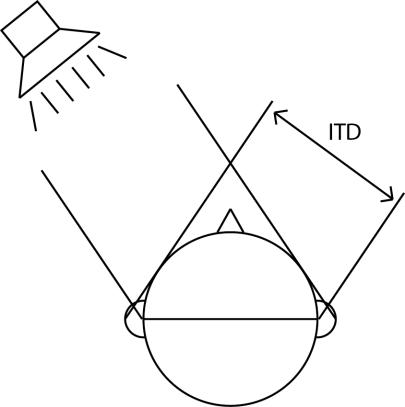
\includegraphics[width=150px]{img/ITD.jpg}
  \caption{TLS (angl. \textit{ITD}) efektas}
  \label{fig:ITD_1}
\end{figure}

Tačiau išimtį sudaro garsas esantis tiesiai prieš arba už klausytojo. TLS taip pat įtakoja garso bangos fazės  pakitimą. Jeigu fazių skirtumas didesnis nei 180 laipsnių, nustatyti kaip fazė yra pasislinkus tampa sunku. Žemuose dažniuose fazės skirtumas nusako pakankamai didelį laiko skirtumą ir yra naudingas orientacijos nustatymui. Aukšto dažnio signalams 180 laipsnių fazės poslinkis  nusakys mažesnį laiko skirtumą. Tai reiškia kad ši savybė tampa mažiau naudinga garso bangoms kurių dažnis priklausomai nuo kampo viršija 700-1500 Hz.

\subsection{Tarpausinis garso lygių skirtumas}
TGLS nusako garso stiprumo skirtumą tarp dviejų taškų (ausų). Šis reiškinys pasireiškia kai garso banga iš dalies yra blokuota galvos. Taip pat kaip ir TLS, TGLS negali tiksliai nusakyti skirtumo tarp garso esančio tiesiai prieš arba už klausytojo. TGLS efektas taipogi kaip ir TLS turi dažninę priklausomybę. Žemuose dažniuose dėl difrakcijos tik maža garso bangos dalis yra blokuota galvos, ko pasėkoje garso intensyvumo skirtumas pasidaro labai mažas.

Tačiau aukštų dažnių ruože difrakcija pasireiškia žymiai mažiau kas įtakoja žymiai didesni garso lygių skirtumą (\ref{fig:ILD_1} paveikslas). Kai kuriais atvejais garso lygių skirtumas gali sudaryti iki 20 dB. Todėl TGLS yra dažniausiai naudojamas aukšto dažnio garso bangoms, o TLS žemo dažnio bangų krypčiai nustatyti. 

\begin{figure}[!h]
  \centering
  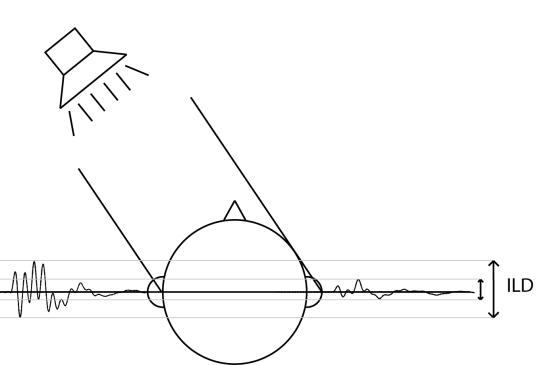
\includegraphics[width=150px]{img/ILD.jpg}
  \caption{TGLS (angl. \textit{ITD}) efektas}
  \label{fig:ILD_1}
\end{figure}

Taipogi labai svarbi yra spektrinė dedamoji (angl. \textit{pinnae effect}). Dėl kompleksinės ir asimetrinės ausies kriauklės formos garsas atsispindėjęs nuo ausies kriauklės spektriškai pasikeičia.  Kartu su pečių atspindžio efektu tai formuoja filtrą turintį krypties priklausomybę ir todėl ne taip kaip TLS ir TGLS yra įmanoma atskirti garsus sklindančius iš priekio ir iš galo. Dėl spektrinių pokyčių ši dedamoji geriausiai tinka atskirti plačiajuostį garsą - viršijantį 6 kHz dažnį.


\subsection{HRTF metodo panaudojimas}

Norint panaudoti šį metodą reikia turėti \textit{HRTF} rinkinį visiems vertikalių ir horizontalių kampų deriniams. Šiame darbe naudojami Masačiuseco technologijų instituto (angl. \textit{Massachusetts Institute of Technology}) 1994 metais atlikto projekto \textit{„KEMAR“} metu gauti universalūs \textit{HRTF} deriniai.

Turint baigtinio ilgio skaitmeninį garso signalą atliekama diskrečioji sąsuka (angl. \textit{convolution}) pagal sekančią formulę:

\begin{equation}
(f * g)[n] = \sum_{m=0}^{\infty} f[m]*g[n-m]=\sum_{m=0}^{\infty} f[n-m]*g[n]
\end{equation}

čia $f$ – vieno kanalo baigtinio ilgio daugianaris (angl. \textit{polynomial}), $g$ – atitinkamo kanalo \textit{HRTF} funkcija (išreikšta daugianariu), $n$ – daugianario narių skaičius.

Šioje formulėje atliekama dviejų daugianarių daugyba, rezultate gauto daugianario koeficientai atitinka originalaus daugianario ($f$) koeficientų seką po sąsukos, visi likę nežinomi koeficientai yra prilyginami nuliui kad nekiltų neapibrėžtumas. Šis veiksmas dar žinomas kaip dviejų daugianarių koeficientų Kauči daugyba (angl. \textit{Cauchy product}).

Veiksmas atliekamas atskirai dešiniajam ir kairiajam kanalams naudojant tą patį garso signalą su atitinkamai dešiniajai arba kairiajai ausiai skirta \textit{HRTF} funkcija.

\subsection{Duplekso teorija}

Duplekso teorija, pateikta Lordo Reilėjaus (Lord Rayleigh), pateikia paaiškinimus apie žmogaus galimybę lokalizuoti garsus pagal laiko skirtumą TLS tarp garsų, patenkančių į kiekvieną ausį ir taip pat skirtingo garso lygio TGLS patekimą į ausis. Bet iki šiol išlieka klausimas, ar šie skirtumai yra pastebimi.

Duplekso teorija teigia, kad TLS naudojamas žemo dažnio garso šaltinio lokalizacijai, o TGLS – aukšto dažnio. Kadangi natūralus garsas sudarytas ne tik iš žemo dažnio komponenčių, bet ir aukšto dažnio, tai klausos sistema turės panaudoti abi metodikas (tiek TLS tiek TGLS), norint tiksliai nustatyti garso šaltinio vietą. Šios dupleksinės sistemos rezultatas – ji gali taip pat generuoti taip vadinamus „garso lokalizacijos užuominų mainų“  arba „laiko intensyvumo mainų“ dirgiklius ausinėse, kur TLS, nukreiptas į kairiąją ausinių pusę, perstumtas per TGLS, kuris savo ruoštu nukreiptas į dešiniąją ausinių dalį, todėl garsas suvokiamas lyg sklistų iš vidurio. Kaip ir visos teorijos, duplekso teorija taip pat susiduria su problemomis. Pastaroji negali iki galo paaiškinti kryptingo girdėjimo, o taip pat išlieka priekinio-galinio garso šaltinio padėties girdimumo problema. Taip pat ši teorija apima tik horizontaliąją garso šaltinio lokalizaciją aplink galvą. Dar vienas teorijos netikslumas – neatsižvelgimas į ausies kaušelio formą lokalizacijos paaiškinime.

1938 metais Vudvortas atliko eksperimentą, kuriame iš pilnavidurio rutulio buvo sumodeliuota žmogaus galva. Su šiuo modeliu buvo matuojami LS kaip kampo su vertikalia plokštuma funkcija skirtingiems dažniams. Šiame galvos modelyje tarpas tarp dviejų ausų buvo apie 22-23 cm. Pirminiai testo rezultatai parodė, kad didžiausias laiko tarpas per kurį garsas patenka iš vienos ausies į kitą buvo apie 660 μs, kai garso šaltinis buvo padėtas lygiai 90O kampu vertikalios plokštumos atžvilgiu. Šis laiko tarpas koreliuojasi su 1500 Hz dažnio garso bangos ilgiu. Rezultatai parodė, jog grojant garsui, kurio dažnis mažesnis nei 1500 Hz bangos ilgis yra didesnis negu minėtojo didžiausio laiko tarpo. Taigi rezultatai parodo, jog tarp garso bangų patenkančių į ausis atsiranda fazių skirtumas ir tai sukuria akustinės lokalizacijos užuominas. Garso dažniui artėjant prie 1500 Hz garso bangos ilgis yra panašus į natūralų garso vėlavimą. Dėl galvos dydžio ir tarpo tarp ausų yra sumažėjęs fazių skirtumas, taigi iš karto atsiranda lokalizacijos paklaida. Garso dažniui esant didesniam nei 1500 Hz garso bangos ilgis tampa mažesnis nei atstumas tarp ausų, tuomet atsiranda „galvos šešėlis“ ir GLS suteikia garso lokalizacijos užuominų.

Feddersen et al. taip pat atliko eksperimentus (1957 metais), kuriais jis matavo kaip kinta LS keičiant garsiakalbio kampą su vertikaliąja plokštuma aplink galvą esant skirtingiems dažniams. Bet jo eksperimentai skyrėsi nuo „Woodworth“ tuo, kad Feddersen‘as atliko tyrimus su realiai žmonėmis, o ne su galvos modeliais. Testo rezultatai sutapo su „Woodworth“ gautais rezultatais. Tyrimo rezultatai taip pat parodė, kad nėra jokio LS skirtumo tarp dviejų garso šaltinio pozicijų – kai garso šaltinis yra prie žmogaus galvą (90) ir už galvos (180). Tokie rezultatų paaiškinimas – garso šaltinio atstumas iki ausų yra vienodas abiem atvejais. Laiko skirtumas keičiasi tik garso šaltiniui keliaujant aplink galvą. Šiuo testu įrodyta, kad didžiausias laiko skirtumas – 660 μs gaunamas garso šaltinį padėjus 90 kampu prie vienos ausies.

\ref{fig:ITD_1} pav. matoma, jog kelio skirtumas nuo garso šalinio iki kiekvienos ausies yra skirtingas. Garso kelias iki kairės ausies yra didesnis nei kelias iki dešinės ausies. Šis garso kelių skirtumas perkeltas į lauko ašį nusako tarpausinį laiko skirtumą (ang. \textit{ITD}, trump. LS).
LS yra dominuojanti užuomina dažniams iki 1.5 kHz (imtinai). Visiems kitiems dažniams didesniems nei 1.5 kHz dominuojanti užuomina yra tarpausinis garso lygio skirtumas (ang. \textit{ILD}, trump. GLS). Tarpausinis garso lygio skirtumas atsiranda dėl taip vaidinamojo galvos šešėlio. Jis atsiranda tik prie aukštesnių dažnių, kuomet garso bangos nebesukelia difrakcijos aplink galvą, taip sukurdamos galvos šešėlį, kuris panašus į šešėlį susidarantį krentant šviesos bangoms link galvos.
Norint įrodyti Lordo Reileigo teoriją, buvo atliktas eksperimentas, kuriame garso šaltinį ir manekeno galvą skyrė 1,75 m. Eksperimentas atliktas beaidėje aplinkoje. Jį atliko Levisas Skotas Diamondas (\textit{Lewis Scott Diamond}).  Naudojant skirtingo dažnio – 125 kHz, 250 kHz, 500 kHz ir 1000 kHz programa Csound sugeneruotus garsus, kai garso signalo šaltinis buvo padėtas skirtingais kampais – 0, 10, 30, 50, 70, 90, pavyko įrodyti šią teoriją.



\end{document}